%!Tex Root = ../main.tex
% ./Packete.tex
% ./Design.tex
% ./Deklarationen.tex
% ./Vorbereitung.tex
% ./Aufgabe1.tex
% ./Aufgabe3.tex
% ./Aufgabe4.tex
% ./Appendix.tex

\section{Aufgabe 2}

\setcounter{exercise}{1}

\begin{frame}[allowframebreaks]{Aufgabe \thesection}{Formale Beschreibung von Schaltkreisen}
  \begin{solution}
    \centering
      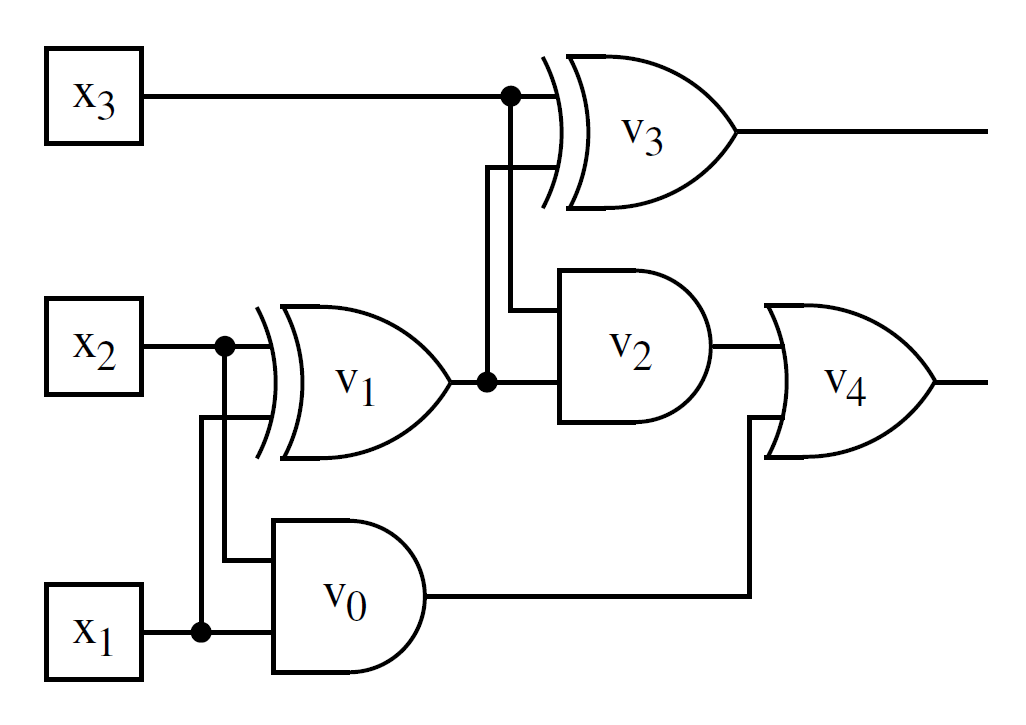
\includegraphics[width=130pt]{figures/Schaltkreis.png}
  \end{solution}
  \begin{solution}
    \centering
      \begin{tabular}{c|c}
        Gatterausgang&Funktion\\ \hline
         $v_0$&$x_1\wedge x_2$\\
         $v_1$&$x_1\oplus x_2$\\
         $v_2$&$(x_1\oplus x_2)\wedge x_3$\\
         \hline
         $v_3$&$(x_1\oplus x_2)\oplus x_3$\\
         $v_4$&$(x_1\wedge x_2)\vee((x_1\oplus x_2)\wedge x_3)$\\
    \end{tabular}
  \end{solution}
  \begin{solution}
      $depth(C)=3$, über den Pfad $v_1,v_2,v_4$
  \end{solution}
\end{frame}
